\documentclass{article}

\usepackage{Sweave}
\begin{document}
\Sconcordance{concordance:simulations.tex:simulations.Rnw:%
1 2 1 1 0 7 1 1 2 5 0 1 3 1 2 1 0 1 1 3 0 2 2 1 0 1 1 3 0 1 2 1 1 1 3 2 %
0 2 1 7 0 1 6 1 2 1 0 1 2 4 0 1 2 1 1 1 -3 1 7 5 1 1 5 8 0 1 3 1 1 1 2 %
1 0 1 1 3 0 1 2 1 1 1 -3 1 7 5 1 1 2 1 0 1 1 3 0 1 2 1 1 1 -3 1 7 4 1 1 %
2 1 0 1 1 3 0 1 3 1 1 1 -4 1 8 4 1 1 2 1 0 1 2 1 0 1 1 3 0 1 2 2 1 2 2 %
4 1 1 3 11 0 1 3 1 1 1 2 10 0 1 3 1 2 4 0 1 2 4 1 1 6 1 3 5 1}


\title{Simulations for two-dimensional distance sampling with time}
\author{David L. Borchers and Martin J. Cox}
\maketitle
\section{Set-up}
\subsection{Load packages and code and set-up}
\begin{Schunk}
\begin{Sinput}
> source("~/dropbox/packages/2D distance sampling with time/R/2D_LT_functions V2a1.r")
> 
\end{Sinput}
\end{Schunk}
Set-up maximum distances:
\begin{Schunk}
\begin{Sinput}
> ystart=3 #maximum y-dimension distance
> w=1  #truncation distance
\end{Sinput}
\end{Schunk}
Set-up survey grid
\begin{Schunk}
\begin{Sinput}
> gridx=seq(w/100,w,length=100)
> gridy=seq(ystart/100,ystart,length=100)
\end{Sinput}
\end{Schunk}
\subsection{Specifications for true animal density} 
True variation in animal density with respect to the track line is defined by \texttt{pi.x}:
\begin{Schunk}
\begin{Sinput}
> ##Truncated normal 
> mu.pi=0#0.5
> sd.pi=0.2
> pi.x=pi.norm; logphi=c(mu.pi,log(sd.pi))
> ##Uniform:
> #pi.x=pi.const; logphi=c(1,NA)
> ##Hazard rate - form 2
> #pi.x=pi.hr2; logphi=log(c(0.75,1))
\end{Sinput}
\end{Schunk}
NB hazard rate density is used to test the MLE to ensure the density distribution can be disentangled from the detection function -  we can assume perfect detectability and a hazard density distirbution, then obtain MLE results.  The selected true perpendicular density \texttt{pi.x}, with parameters \texttt{logphi} is shown in Fig. \ref{fig:perp.den}.
\begin{Schunk}
\begin{Sinput}
> adbn=pi.x(gridx,logphi,w)
> plot(gridx,adbn,type="l",ylim=c(0,max(adbn)),
+      xlab="perp dist (x)",ylab="pi(x)")
\end{Sinput}
\end{Schunk}
\begin{figure}
\begin{centering}
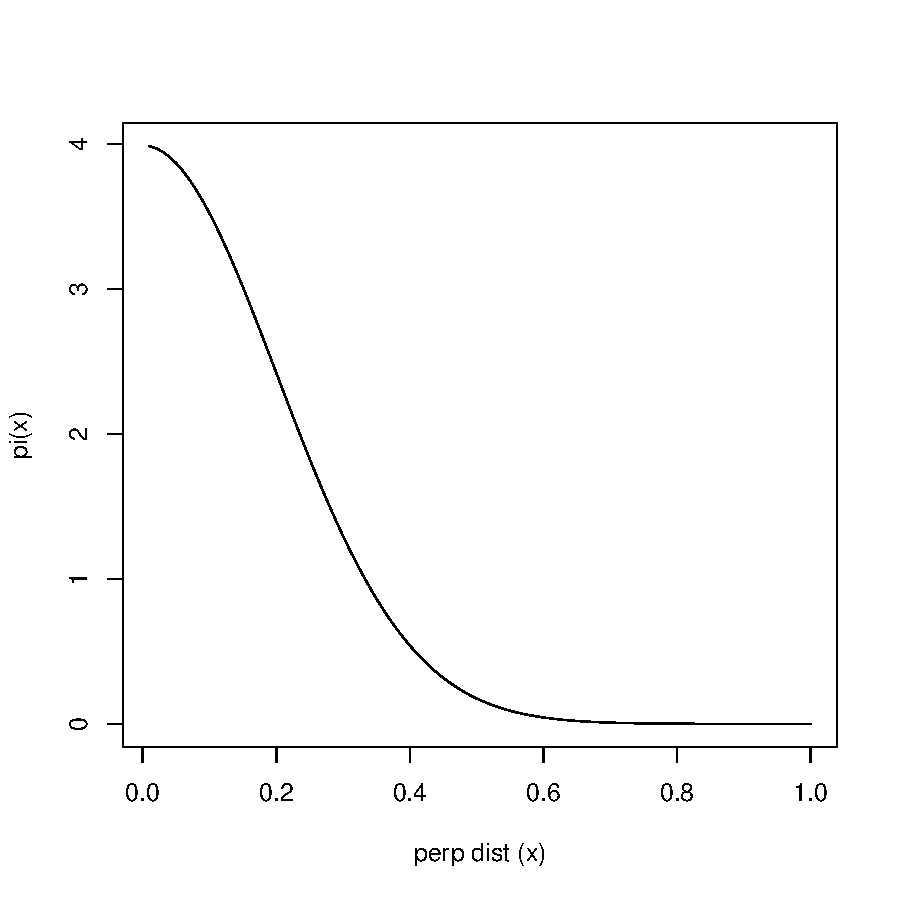
\includegraphics{simulations-figDen}

\caption{Perpendicular density distribution, $\pi(x)$ as specified in \texttt{pi.x} and parameters \texttt{logphi}.} \label{fig:perp.den}
\end{centering}
\end{figure}
\subsection{Hazard rate}
The true hazard rate function is specified using:
\begin{Schunk}
\begin{Sinput}
> #hr=h1; b=log(c(0.75,0.2))
> #hr=h1; b=log(c(0.001,1))
> #hr=h.okamura; b=log(c(50,25))
> hr=h2; b=log(c(0.75,1)) # this produces a sensible h-r p(x) shape
> #hr=h.const; b=c(1,NA)
\end{Sinput}
\end{Schunk}
The selected true hazard function \texttt{hr}, with parameters \texttt{b} is shown in Fig. \ref{fig:hr}.

\begin{Schunk}
\begin{Sinput}
> haz=outer(gridx,gridy,FUN=hr,b=b)
> persp(gridx,gridy,log(haz),theta=45,phi=35)
\end{Sinput}
\end{Schunk}
\begin{figure}
\begin{centering}
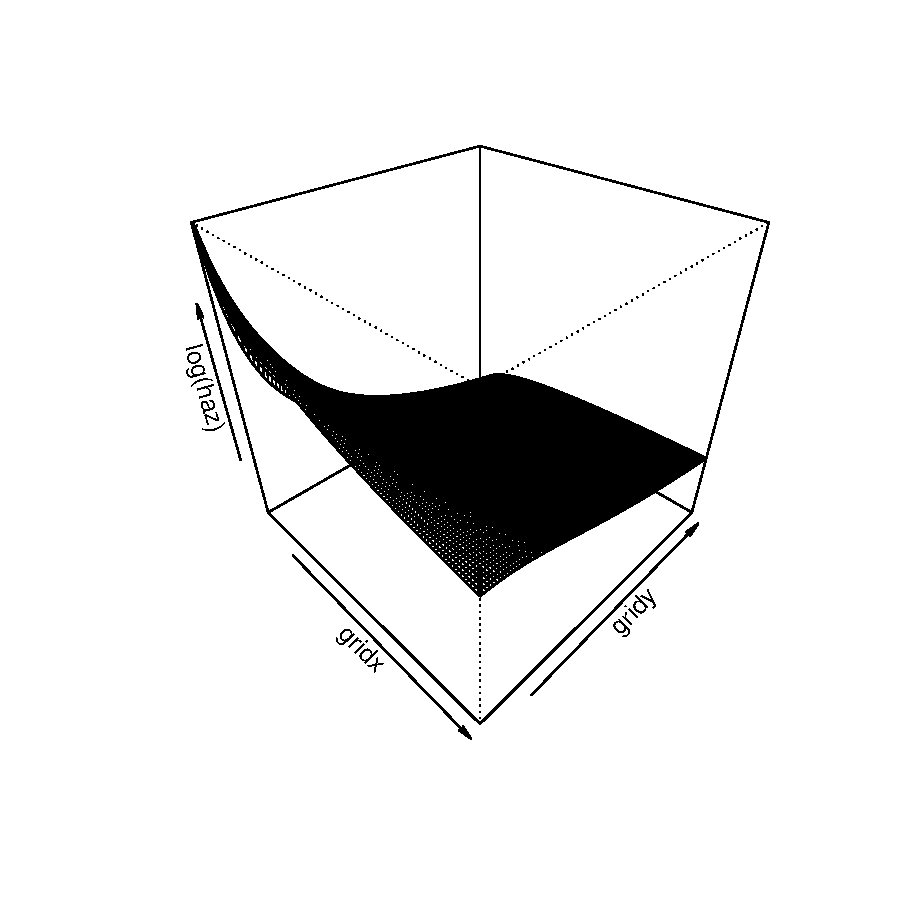
\includegraphics{simulations-fighr}

\caption{Hazard rate function, $h(y|x)$, displayed on the $\log$ scale as specified in \texttt{pi.x} with parameters \texttt{b}.} \label{fig:hr}
\end{centering}
\end{figure}
A pdf of \emph{waiting distance} - the $y$-dimension distance when detections occur - $f(y|x)$ across the $x,y$ grid is given in Fig. \ref{fig:wait}.

\begin{Schunk}
\begin{Sinput}
> f=outer(gridy,gridx,FUN=fyx,b=b,hr=hr,ystart=ystart)
> persp(gridx,gridy,t(f),theta=45,phi=35,zlim=c(0,max(f)),zlab="f(y|x)")
\end{Sinput}
\end{Schunk}
\begin{figure}
\begin{centering}
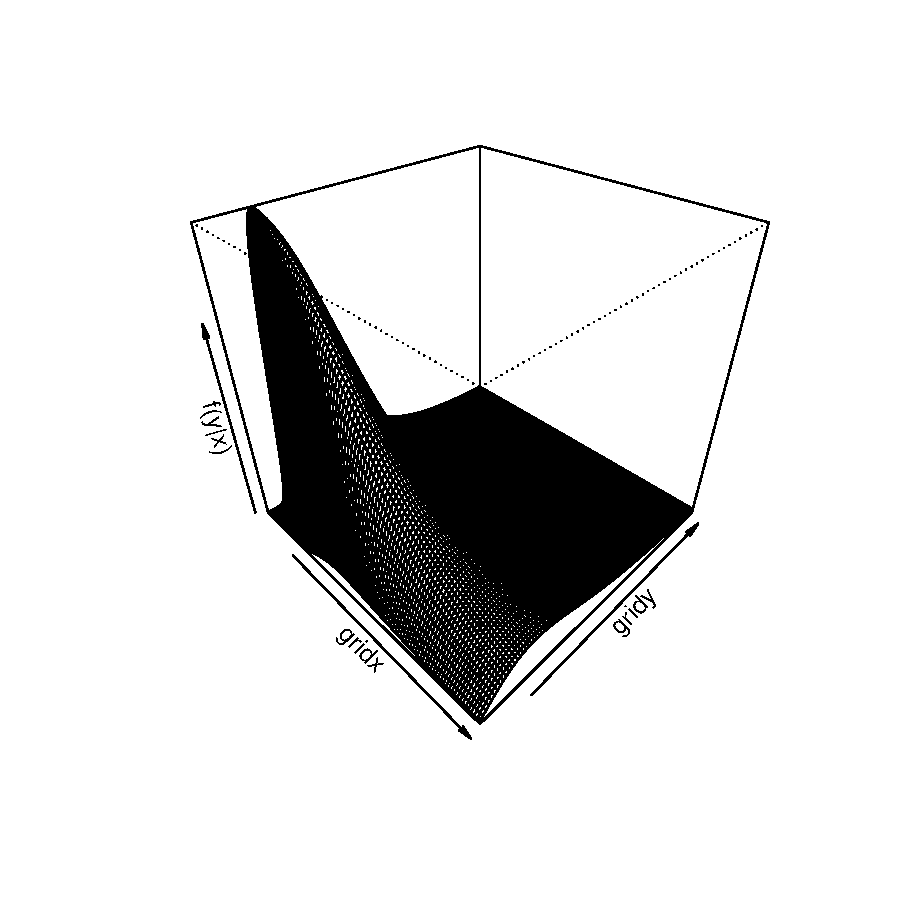
\includegraphics{simulations-figwait}

\caption{PDF of waiting distance, $f(y|x)$.} \label{fig:wait}
\end{centering}
\end{figure}
and the survival function $p(x)$ is given in Fig. \ref{fig:sur}.
\begin{Schunk}
\begin{Sinput}
> p.x=px(gridx,b,hr,ystart,nint=100)
> plot(gridx,p.x,type="l",ylim=c(0,max(p.x)),xlab="prep. distance, x",ylab="p(x)")
\end{Sinput}
\end{Schunk}
\begin{figure}
\begin{centering}
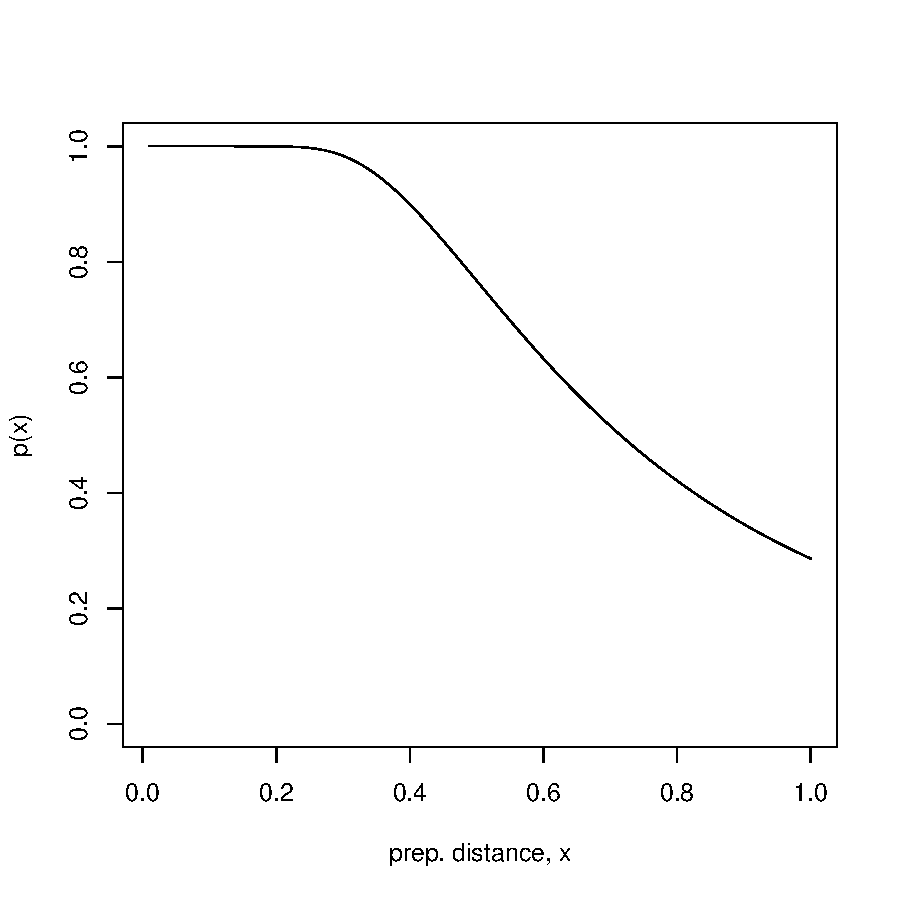
\includegraphics{simulations-figsur}
\caption{Survival function, $p(x)$.} \label{fig:sur}
\end{centering}
\end{figure}
\section{Simulating sightings}
Now we have specified a survival function and density distribution we can simulate sightings from a known population of $N$ animals:
\begin{Schunk}
\begin{Sinput}
> N=50
> simRes=simXY(N=N,pi.x=pi.x,logphi=logphi,
+               hr=hr,b=b,w=w,ystart=ystart)
> x=simRes$locs$x; y=simRes$locs$y 
\end{Sinput}
\end{Schunk}
and plot the results (Fig. \ref{fig:simXY}).
\begin{figure}
\begin{centering}
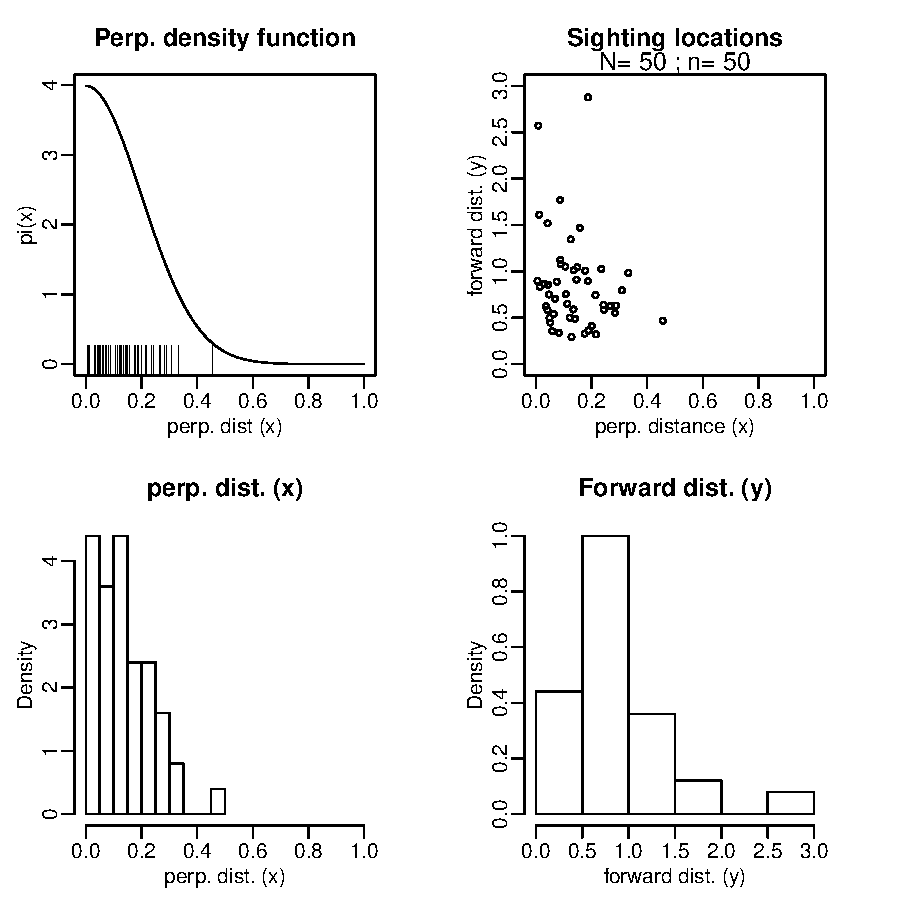
\includegraphics{simulations-figXYsim}
\caption{Simulated positions.} \label{fig:simXY}
\end{centering}
\end{figure}
\section{Maximum likelihood estimation}
Now we have specified a true hazard function, $h(y|x)$ (R object \texttt{hr}) and perpendicular density distribution $\pi(x)$ (R object \texttt{pi.x}) and simulated sightings (R objects \texttt{x} and \texttt{y}), we can use our maximum likelihood to estimate parameters for $h(y|x)$ and $\pi(x)$.  In our first example, we use the known forms of $h(y|x)$ and $\pi(x)$ and use their true parameters as starting values:
\begin{Schunk}
\begin{Sinput}
> #(pars=c(b,logphi))
> (pars=c(b,0.3,-1.2))
\end{Sinput}
\begin{Soutput}
[1] -0.2876821  0.0000000  0.3000000 -1.2000000
\end{Soutput}
\begin{Sinput}
> 
\end{Sinput}
\end{Schunk}

The negative log-likelihood function that we will maximise is:
\begin{Schunk}
\begin{Sinput}
> (negloglik.yx(y,x,pars,hr,ystart,pi.x,w))
\end{Sinput}
\begin{Soutput}
[1] 0.4922518
\end{Soutput}
\begin{Sinput}
> 
\end{Sinput}
\end{Schunk}
and is maximised here:
\begin{Schunk}
\begin{Sinput}
> est.yx=fityx(y,x,b,hr,ystart,pi.x,logphi,w)#,control=list(trace=5))
\end{Sinput}
\end{Schunk}
\section{Results}


\begin{figure}
\begin{centering}
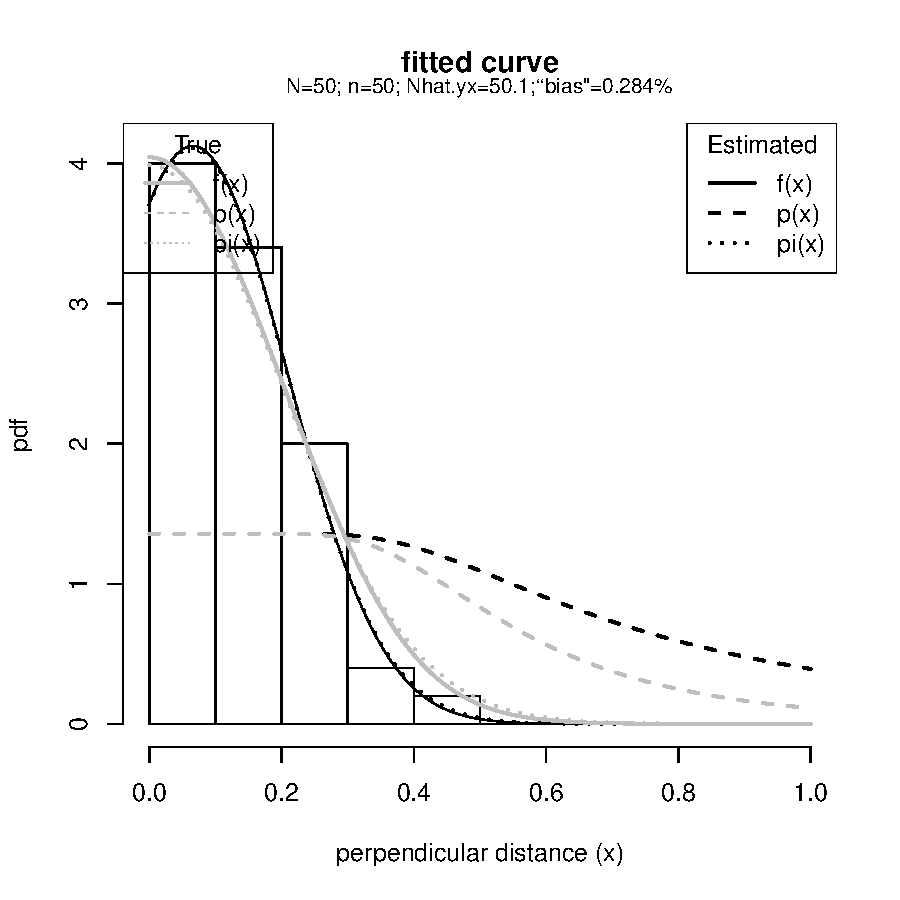
\includegraphics{simulations-plotMLE}
\caption{Maximum likelihood fit.} \label{fig:mleFit}
\end{centering}
\end{figure}
The resulting fit is plotted in Fig. \ref{fig:mleFit}, and from a population of $N$ = 50 animals, of which $n$ = 50 were seen, the MLE gave $\hat{N}$= 50.1 and was 0.284\% biased.

\end{document}
